\section{Replication Consensus Algorithm: Raft}
As we've discussed so far, replication consistency is crucial and a 
difficult task. The next strategy, \textbf{Raft}, deals with such problem.
There are other solutions, however, Raft is considered safe and easier to 
implement correctly than other solutions. First we must familiarize ourselves with the following terms:
\begin{Def}[State Machines in Distributed Systems]
    
    A \textbf{State Machine} processes \underline{deterministic} sequence of inputs from a \textbf{log} and saves them
    in state.
    \textbf{Replicated state machines} are implemented via \textbf{replicated logs} across multiple servers
    utilizing a \textbf{Consensus Algorithm}, which validates log order.
\end{Def}

\vspace{-1em}
\begin{figure}[h]
    \centering
    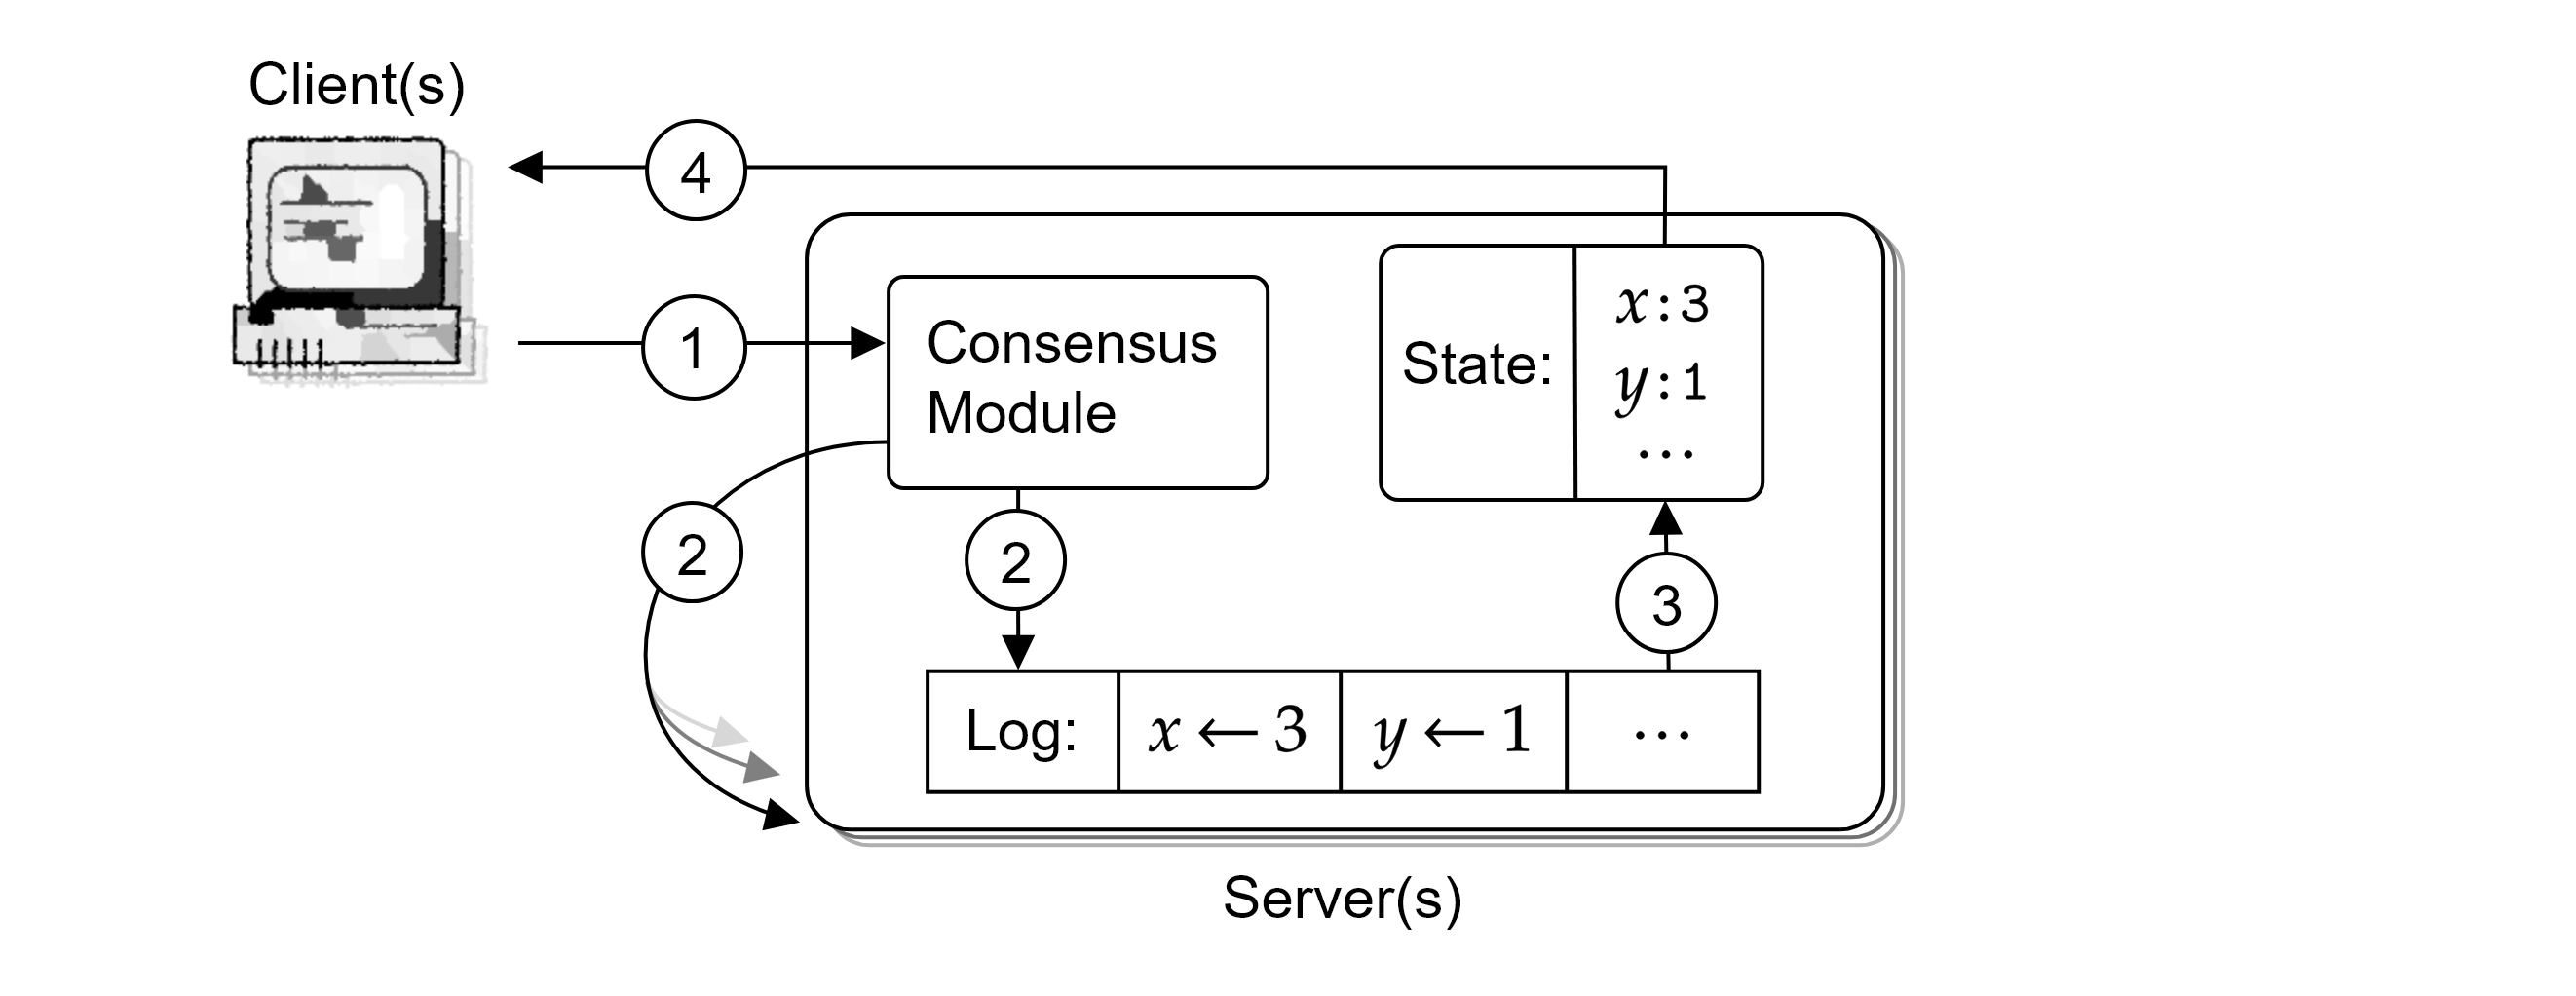
\includegraphics[width=1\textwidth]{Sections/raft/state.png}
    \caption{High-level framework for replicated state machines.}
\end{figure}
\noindent
In the above the \textbf{Consensus Module} communicates with other servers to serve consistent logs. 

\newpage 

\noindent
Now to define the parts which make up a consensus algorithm:
\begin{Def}[Consensus Algorithm Components]

    A \textbf{Consensus Algorithm} involves the following components:
    \begin{itemize}
        \item \textbf{Safety}: Always returns correct results in spite, network delays, partitions, duplications, and reorderings.
        \item \textbf{Liveness}: A \textbf{Cluster} (group of servers) must tolerate a subset of server failures (e.g., A cluster of 5 servers can tolerate 2 failures). Offline 
        servers may later recover and rejoin the cluster.
        \item \textbf{Time Agnostic}: The algorithm must not rely on synchronized clocks.
        \item \textbf{Majority Rule}: A majority of servers must agree on a value before it is committed. Minority slow servers must not block the system.
    \end{itemize}
\end{Def}

\noindent
At a high level, The Raft Algorithm:
\begin{Def}[Raft Abstract]

    The Raft Algorithm involves three main components:
    \begin{itemize}
        \item \textbf{Leader Election}: A leader $\ell$ is elected to manage the replication process of backups $\beta$.
        \item \textbf{Heartbeats}: Where $\ell$ and $\beta$ exchange consistent pulses of data to ensure liveliness.
        \item \textbf{Assurance}: Commit points (\ref{def:commit}) are established between the client, $\ell$, and $\beta$. 
    \end{itemize}
\end{Def}
\noindent
In Raft, servers are given roles to manage the replication process.
\begin{Def}[Raft Server States]

    A Raft server can be in one of the following states:
    \begin{itemize}
        \item \textbf{Follower}: A server that listens to the leader.
        \item \textbf{Candidate}: A server that is running for leader.
        \item \textbf{Leader}: A server that is managing the replication process.
    \end{itemize}
    \textbf{Followers are passive} and simply listen to the leader. \textbf{Clients interact with the leader}. Followers that are contacted \textbf{will redirect} the request to the leader.
\end{Def}
